\documentclass{article}

\usepackage{amsmath}
\usepackage{amsfonts}
\usepackage{graphicx}
\usepackage{float}
\usepackage{hyperref}
\usepackage[margin=0.75in]{geometry}

\graphicspath{{./assets/}}

\title{Output voltage of potential divider | Interpreting analog signals from resistive sensors}
\author{Igor Krzywda}

\begin{document}

\maketitle

\section{Introduction}

    Voltage divider is an ubiquitous and vesrsitaile electric component. It consists of two resistors connected 
    in series with output terminal between them (See Figure~\ref{fig:divider_0}. All resistive sensors in its core are 
    voltage dividers, where the sensor itself is one of the resistors in a circuit allowing for reading analog signal from them, 
    as the sensor changes its resistance in accordance to some external variable like light, reaction force or
    temperature. What potential dividers are not good for is providing power to a load, which, along with reading information
    will be explored in this paper.

    \begin{figure}[H]
        \caption
        \centering
        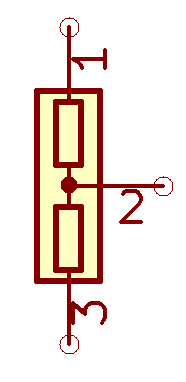
\includegraphics[width=0.1\linewidth]{divider_0}
        \label{fig:divider_0}
    \end{figure}

\section{Output voltage of a potential divider without load}

    The output voltage of a voltage divider is measured across $R_2$ (Figure~\ref{fig:divider_0}, so the formula for the output
    can be derived from Ohm's law

    \begin{align}
        V_{out} = IR_2 \\
        I = \frac{V_{in}}{R_1 + R_2} \\
        V_{out} = \frac{V_{in}R_2}{R_1 + R_2} \label{eq:div_wo_load} 
    \end{align}

    From equation above, we can already see that output of resistive sensors is not linear (except in the case of potentiometer, 
    where the resistance of the whole system is fixed). Another thing to be seen is that by adjusting $R_1$ we can set the resolution
    of a sensor...

\section{Output voltage of a potential divider under load}

    \begin{figure}[H]
        \caption
        \centering
        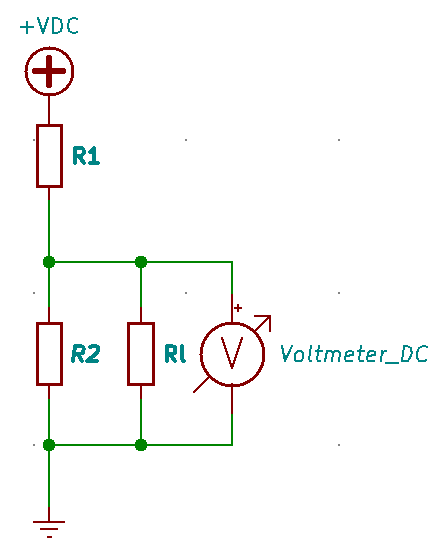
\includegraphics[width=0.3\linewidth]{divider_1}
        \label{fig:divider_1}
    \end{figure}

    Figure~\ref{fig:divider_1} shows the model the analysis is build upon, where $R_1$ and $R_2$ are
    resistors of the potential divider, $R_l$ is the resistive load and $V_{out}$ being measured using
    the voltmeter.

    If a resistive load were to be connected to a potential divider, then it may be interpreted as
    if the connected resistor with load in paralel were one resistor connected in series. The formula
    for resistance in a parallel circuit is stated in equation~\eqref{parallel_circuit_R}.

    \begin{equation}\label{parallel_circuit_R}
        \frac{1}{R} = \frac{1}{R_1} + \frac{1}{R_2} + ... + \frac{1}{R_n}
    \end{equation}
    
    From that equation we can state that if any load were to be connected to the divider, the net 
    resistance of $R_2$ and $R_l$ is going to be lower than one of sole $R_2$. We can derive the 
    output voltage from equation~\eqref{eq:div_wo_load}
    
    \begin{align}
        R_p = (\frac{1}{R_2} + \frac{1}{R_l})^{-1} = \frac{R_2R_l}{R_2 + R_l} \\
        V_{out} = \frac{V_{in} \cdot R_p}{(R_1 + R_p)} \\
        V_{out} = \frac{V_{in}(R_2R_l)}{R_1(R_2 + R_l) + R_2R_l} \label{ohm_derived}
    \end{align}

\end{document}
